%%%% Arquivo base para o documento - ver. 1.00 (24/02/2016)
% % % % % % % % % % % % % % % % 
%%%%%%MDT UFSM 2015%%%%%%%%%%%%
% % % % % % % % % % % % % % % % 

% % % % % PAGINACAO
\documentclass[oneside,openright,12pt]{ufsm_2015} %%%%% <100 páginas
%\documentclass[twoside,openright,12pt]{ufsm_2015} %%%% >100 páginas

%%%%% PACOTES %%%%%
\usepackage{amsmath}
\usepackage{enumerate}
\usepackage{amssymb}
\usepackage{graphicx}
\usepackage{epsf,amsfonts}
\usepackage{amsfonts}
\usepackage{epstopdf}
\usepackage{float}
\usepackage{mhchem}
\usepackage[utf8]{inputenc}  %utf8
% \usepackage[latin1]{inputenc}   %europeu
\usepackage[brazil]{babel}
\usepackage[T1]{fontenc}
\usepackage{indentfirst}
\usepackage{textcomp}
\usepackage{setspace}
\usepackage{picinpar}
\usepackage{ifthen}
\usepackage{path}
\usepackage{scalefnt}
\usepackage{tocloft}
\usepackage[overload]{textcase}

%%%%% FIM PACOTES %%%%%

%%%%% DADOS INICIAIS %%%%%

\centroensino{Centro de Tecnologia}  %%% NOME POR EXTENSO
\centroensinosigla{CT}  %%% SIGLA
\nivelensino{Graduação}  %%%%%%% NIVEL DE ENSINO 
\curso{Sistemas de Informação}   %%%%% NOME POR EXTENSO
\ppg{PPGALGO}   %%%%%% SIGLA
\statuscurso{Curso}  %%%% STATUS= {Programa} ou {Curso}

% % % % % % % % % % INFORMACOES DO AUTOR % % % % % % % % % % 
\author{Marinara Rübenich Fumagalli}   %%%%% AUTOR DO TRABALHO
\sexo{F} %%%% SEXO DO AUTOR -> M=masculino   F=feminino (IMPORTANTE PARA AJUSTAR PAGINAS PRE-TEXTUAIS)
\grauensino{Graduação}    %%%%%%%% GRAU DE ENSINO A SER CONCLUIDO
\grauobtido{Bacharela}    %%%%% TITULO OBTIDO
\email{mrfumagalli@inf.ufsm.br}   %%%% E-MAIL
%\endereco{Rua Mato Grosso, n. 119}
%\fone{55 99648 6140}

% % % % % % % % % % INFORMACOES DA BANCA % % % % % % % % % % 
\orientador{Joaquim Vinicius Carvallho Assunção}{Dr}{UFSM}{M}{P}  
\bancaum{Banca Um}{Dr}{UFSM}{F}{M}  %%%INFORMACOES SOBRE PRIMEIRO 
\bancadois{Banca Dois}{Dr}{UFSM}  %%%INFORMACOES SOBRE SEGUNDO
\bancatres{Banca Três}{Dra}{UFSM} %%%INFORMACOES SOBRE TERCEIRO 

% % % % % % % % % % INFORMACOES SOBRE O TRABALHO % % % % % % % % % %
% % % %  TITULO DO TRABALHO
\titulo{Aplicação de Redes Neurais para estimativa de temperaturas com base em amostras de foraminíferos}
\englishtitle{Application of Neural Networks to estimate temperatures based on foraminifera samples}
\tfg  %% Trabalho Final de Graduacao (nao exibe area de concentracao)
% % % DATA DA DEFESA 
\data{08}{07}{2019} %% FORMATO {DD}{MM}{AAAA}

% % % % %  ALGUMAS ENTRADAS PRE-TEXTUAIS
% % % EPIGRAFE
\epigrafe{"Os animais são meus amigos e eu não como meus amigos"}{George Bernard Shaw}
\epigrafe{"Quando o homem aprender a respeitar até o menor ser da Criação, seja animal ou vegetal, ninguém precisará ensiná-lo a amar seu semelhante"}{Albert Schweitzer}
\epigrafe{“A natureza pode suprir todas as necessidades do homem, menos a sua ganância.”}{Mahatma Gandhi}
% % % DEDICATORIA
\dedicatoria{Dedico este trabalho ao meu pai Carlos, ao meu marido Diego e aos meus cachorrinhos, que considero como filhos, com quem sempre pude contar.
Mas, dedico especialmente à minha mãe, Maria Izabel, a pessoa que mais me incentivou a estudar e que sempre me deu forças quando pensei em desistir.}
% % % %  AGRADECIMENTOS
\agradecimentos{
    Em breve...
}

%%%%% FIM DADOS INICIAIS %%%%%

% % % % %  RESUMO E PALAVRAS CHAVE DO RESUMO
\resumo{
    Foraminíferos são protozoários que vivem nos oceanos, são altamente evolutivos e
    sensíveis às mudanças ambientais. Se apresentam como microfósseis conservados nas rochas
    ou vivos até hoje. Existem milhares de espécies encontradas desde o período cambriano (entre
    542 milhões e 488 milhões de anos atrás). Através da presença deles é possível estimar, dentre
    outros eventos, temperaturas das épocas em que viveram.
    Esta estimativa será dada através da aplicação de redes neurais que são capazes de
    aprender qual a melhor saída baseada em um arquivo de entrada. Neste caso, o arquivo deve
    conter informações de espécies de foraminíferos e a saída será a estimativa da temperatura da
    época em que elas viveram. O resultado será exibido através de uma aplicação web amigável
    ao usuário.
}
\palavrachave{Foraminíferos. Machine Learning. Paleoclima. Redes Neurais.}

% % % % %  ABSTRACT E PALAVRAS CHAVE DO RESUMO - OBRIGATORIO PARA MDT-UFSM
\abstract{
    Abstract here.
}
\keywords{Foraminifera. Machine Leraning. Paleoclimate. Neural Networks.}


% % %  ATIVACAO DE LISTAS E PAGINAS ESPECIAIS
% % LISTA DE FIGURAS 
\semfiguras   %%(QUANDO ATIVIDA NAO EXIBE A LISTA)
% % LISTA DE GRAFICOS 
\semgraficos   %%(QUANDO ATIVIDA NAO EXIBE A LISTA)
% % LISTA DE ILUSTRACOES 
\semilustracoes  %%(QUANDO ATIVIDA NAO EXIBE A LISTA)
% % LISTA DE TABELAS 
\semtabelas   %%(QUANDO ATIVIDA NAO EXIBE A LISTA)
% % LISTA DE QUADROS 
\semquadros   %%(QUANDO ATIVIDA NAO EXIBE A LISTA)
% % LISTA DE APENDICES 
\semapendices  %%(QUANDO ATIVIDA NAO EXIBE A LISTA)
% % LISTA DE ANEXOS 
\semanexos   %%(QUANDO ATIVIDA NAO EXIBE A LISTA)

% % % %  LISTA DE ABREVIATURAS E SIGLAS
%%%%%%%% para não utilizar comente as linhas abaixo.
\siglamax{Rprop} %%%% coloque aqui a maior sigla (indentacao)
\listadeabreviaturasesiglas{
\item[RNA] Redes Neurais Artificiais  
\item[Rprop] Retropropagação Resiliente
\item[UFSM] Universidade Federal de Santa Maria
}

% % % %  LISTA DE SIMBOLOS
\simbolomax{(Re)2} %%%% coloque aqui o maior simbolo (indentacao)
\listadesimbolos{
\item[u_*]  Escala de velocidade de fricção 
\item[w_*]  Escala de velocidade convectiva
\item[(Re)^2] Maior simbolo da lista
}

% % FICHA CATALOGRAFICA
\semcatalografica  %%%%  

% % % % % % % % % % % %  OPCOES DE FORMATACAO % % % % % % % % % % % 
%% helvetica
%\usepackage[scaled]{helvet}
%\renewcommand*\familydefault{\sfdefault}

%% arial
% \renewcommand{\rmdefault}{phv} % Arial
% \renewcommand{\sfdefault}{phv} % Arial

%%times
\usepackage{mathptmx}

 % % % % 
% % % % % % % % % % % %  INICIO DO DOCUMENTO  % % % % % % % % % % % % % % %
\begin{document}

    \pretextual  %%%% GERA AS PAGINAS PRE-TEXTUAIS 
    
    % % % % 
    % % % % % % % % % % INICIO DAS PAGINAS TEXTUAIS % % % % % % % %
    % % % % 
    \introducao{
        \par Insira aqui a introdução!!!
        \par Insira aqui a introdução!!!
    }
    
    \geraintro  %%%% GERA INTRODUCAO
    
    %%%%%%% Início \chapter{Revisão Bibliográfica Crítica} %%%%%%%
    \chapter{Revisão Bibliográfica Crítica}
    
        \par Esta revisão bibliográfica traz definições sobre Foraminíferos e Redes Neurais Artificiais. Conta com 2 seções e 5 subseções: 2.1 Foraminíferos; 2.1.1 Classificação; 2.1.2 Predição de Temperaturas; 2.2 Redes Neurais Artificiais (RNA); 2.2.1 Arquitetura; 2.2.2 Treinamento, Teste e Predição; 2.2.3 Retropropagação Resiliente (RProp); 
        
        %%%%% Início \section{Foraminíferos} %%%%%
        \section{Foraminíferos}
            \par No arquivo modelo de referências, também existem alguns exemplos de diferentes classes de citações. Todas elas podem ser usadas com o \textit{$\backslash$cite$\{$label$\}$} ou \textit{$\backslash$citeonline$\{$label$\}$}, dependendo da forma de citação\footnote{Este é um teste de nota de rodapé}.
          
          \begin{center}\rule{0.5\textwidth}{1pt}\\$\backslash cite\{label1,label2,label3,...\}$\end{center}
        
          \begin{verbatim}
          Os ventos do norte não movem moinhos \cite{tcc:mintegui2014,
          diss:anabor2004, tese:anabor2008, livro:halliday28ed, 
          livro:fedorova:v1, site:amsglo:fog}.
          \end{verbatim}
            
            \begin{center}\rule{0.5\textwidth}{1pt}\\$\backslash citeonline\{label1,label2,label3,...\}$\end{center}
            
            \begin{center}\rule{0.5\textwidth}{1pt}\end{center}   
            
            %%% Início \subsection{Classificação} %%%
            \subsection{Classificação}
                \par A citação \textit{apud} ocorre quando você cita algum autor através de outra obra, sem ter consultado-a propriamente. Neste caso a citação é feita da seguinte forma:
                \begin{center}
                  \rule{0.5\textwidth}{1pt}\\
                  $\backslash apud\{material\_lido\}\{material\_citado\_no\_material\_lido\}$ \\
                \end{center}
                \begin{verbatim}
                    Sobre a circulação geral da atmosfera pode-se dizer que os ventos do norte
                    não movem moinhos \apud{livro:monin:v1}{apud:richardson1922}.
                \end{verbatim}
      
                Sobre a circulação geral da atmosfera pode-se dizer que os ventos do nortenão movem moinhos
                \apud{livro:monin:v1}{apud:richardson1922}.
        
                \begin{center}\rule{0.5\textwidth}{1pt}\end{center} 
                
                \par Nesse caso, na bibliografia só constará a obra consultada e não aquele referenciada pela obra. Para que isso ocorra naturalmente, a obra consultada deve ser incluída normalmente no arquivo referencias.bib enquanto a obra referenciada indiretamente deve ser incluída com a opção \textit{@hidden}, conforme o modelo de referências.
            %%% Fim \subsection{Classificação} %%%
            
            %%% Início \subsection{Estimação de Temperaturas} %%%
            \subsection{Estimação de Temperaturas}
                \par Texto
            %%% Fim \subsection{Estimação de Temperaturas} %%%
        %%%%% Fim \section{Foraminíferos} %%%%%
        
        %%%%% Início \section{Redes Neurais Artificiais (RNA)} %%%%%
        \section{Redes Neurais Artificiais (RNA)}
            \par Texto
            
            %%% Início \subsection{Arquitetura} %%%
            \subsection{Arquitetura}
                \par Texto
            %%% Fim \subsection{Arquitetura} %%%
             
            %%% Início \subsection{Trein., Teste e Predição} %%%   
            \subsection{Treinamento, Teste e Predição}
                \par Texto
            %%% Fim \subsection{Trein., Teste e Predição} %%%
            
            %%% Início \subsection{Retroprop. Resiliente (RProp} %%%
            \subsection{Retropropagação Resiliente (RProp)}
                \par Texto
            %%% Fim \subsection{Retroprop. Resiliente (RProp} %%%
        %%%%% Fim \section{Redes Neurais Artificiais (RNA)} %%%%%
    %%%%%%% Fim \chapter{Revisão Bibliográfica Crítica} %%%%%%%      
    %%%%%%% Início \chapter{Trabalhos Relacionados} %%%%%%%  
    \chapter{Trabalhos Relacionados}
             
         \par Na MDT da UFSM há uma clara diferença entre tabelas e quadros, quanto a sua apresentação. Aqui, para inserir tabelas usa-se o ambiente tradicionalmente definido \textit{table}. A partir deste modelo simples:
             
         \noindent resultando:
             
       \begin{quadro}
          \caption{Modelo de quadro para MTD-UFSM.}
          \centering
          \begin{tabular}{| c |c |c |}
          \hline
          Abacate & Banana & Canela \\
          \hline
          21 & 34 & 56 \\
          \hline
          -3 & 245 & 23 \\
          \hline
          -25 & -0,57 & 2 \\
          \hline
          \end{tabular}
          \vspace{\baselineskip} %%% linha em branco para atendender a norma
            \fonte{Adaptado de \citeonline{livro:halliday28ed}.}
      \end{quadro}
          
    
        \noindent Assim como para as tabelas e figuras, já está definida uma lista de quadros. Além disso, o comando ``fonte'' também pode ser usado aqui se necessário, bem como para figuras. Vale lembrar que, na MDT-UFSM, as legendas de quadros e figuras aparecem embaixo das mesmas. Já nas tabelas, em cima. A fonte sempre embaixo.
             
        \par As figuras devem ser inseridas com o ambiente padrão: \textit{figure}. Veja um exemplo simples:
             
        \begin{figure}[ht]
            \caption{\label{exepretex} Sequência dos elementros pré-testuais da MDT-UFSM}
          \centering
          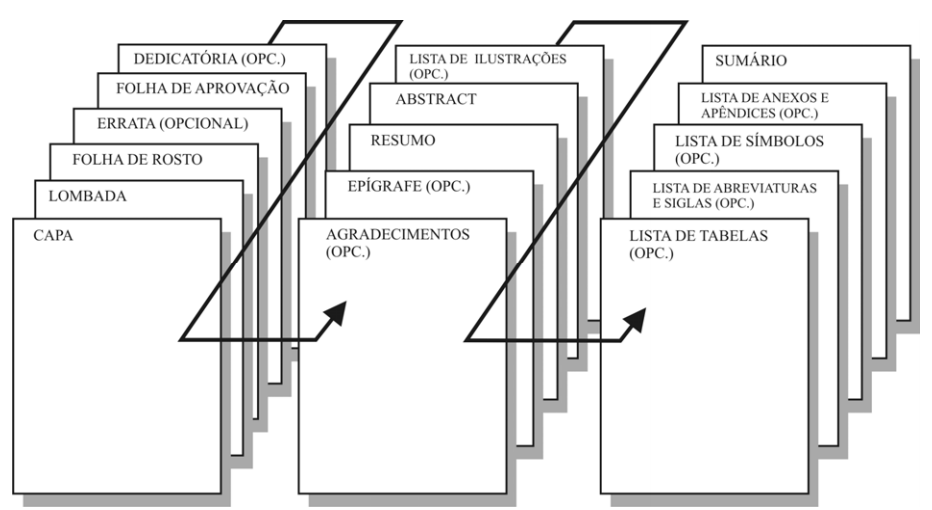
\includegraphics[width=0.6\textwidth]{figuras/pretextuais.png}
          \vspace{\baselineskip} %%% linha em branco para atendender a norma
                \fonte{Adaptado de \citeonline{man:MDTUFSM2012}.}
        \end{figure}
    %%%%%%% Fim \chapter{Trabalhos Relacionados} %%%%%%% 
    
    %%%%%%% Início \chapter{Metodologia} %%%%%%% 
    \chapter{Metodologia}        
    %%%%%%% Fim \chapter{Metodologia} %%%%%%% 
    
    % % % % 
    % % % % % % % % % % % % FIM DAS PAGINAS TEXTUAIS % % % % % % % % % % % % % % 

    %CITAR P/ REFERENCIAR - excluir este capítulo no edito após texto pronto !!!
    \chapter{Citações}
      \citeonline{tcc:gpereira2011, diss:cerentini2018, diss:diaz2014,
      diss:goulart1999, diss:friedrichs2013, tese:pereira2017,
      tese:braga2014, tese:padilha2014, tese:ferraz2013,
      livro:petro2019, livro:petro2018, livro:haykin1994,
      livro:bragacarvalholudemir1998, livro:cushman1948,
      livro:zuurmeestersieno2009, livro:kovacz2006, livro:gurney1997,
      livro:tafnerxerezfilho1995, livro:infante1988,
      livro:haykin2001, livro:silvaspattiflauzino2010,
      livro:sariloesch1996, livro:kovacz1997,
      livro:facelilorenagamacarvalho2011,
      cap:livro:hastietibshiranifriedman2009,
      artigo:saad1996,
      site:ufrgsfora2018, site:uolproto2012}.

    % % % %   
    % % % % % % % % % % % % % BIBLIOGRAFIA  % % % % % % % % % % % % % % % % % % 
    
    \bibliografia{referencias}  %%%%% BIBLIOGRAFIA -> INCLUIR NAS CHAVES O NOME DO ARQUIVO *.BIB  
    
    % % %   
    % % % % % % % % % % % % % APENDICES % % % % % % % % % % % % % % % % % % %
    %\apendice %%%% TEXTOS A PARIR DESTE PONTO SERAO CONSIDERADOS APENDICES
    
    % % % %   
    % % % % % % % % % % % % % % % ANEXOS  % % % % % % % % % % % % % % % % % % %   
    %\anexo    %%%% TEXTOS AQUI SERAO CONSIDERADOS ANEXOS

\end{document} 
 % % % % 
% % % % % % % % % % % %  FIM DO DOCUMENTO  % % % % % % % % % % % % % % %